\chapter{Contextualization and Development Plan} \label{sec:developmentplan}

\section{Context}

In the previous chapter I presented the state of the art of smart shelves. 
To understand the context of the implementation presented throughout the remaining of this dissertation, a brief contextualization of the use case and background is needed.

The smart shelf developed in this dissertation was primarily designed to integrate warehouse storage in Nespresso boutique stores.
Nespresso is a company owned by Nestlé Nespresso S. A., one operational unit of the Nestlé Group, dedicated to the retail and production of coffee capsules, coffee machines and related accessories.
Coffee arrives from different parts of the globe (Colombia, Brazil, Ethiopia, India, Indonesia, to say a few) through seaborne container, reaching the factories by train.
The company has 3 manufacturing facilities producing coffee capsules in Switzerland, from where it dispatches products to supply chain centers.
Coffee machines are manufactured in East Europe and from there, shipped to supply chain centers.
Supply chain centers distribute the products to retail and boutique shops where they are sold~\cite{PortugalRecebeCentro}.

The  complexity  in  the logistics network, due to the growing of the brand, starts to compromise the management of the products down in the chain.
Namely, in boutique stores, the categorization and verification of new inventory, inspection of the arrived goods from the transportation company, returns, control and management of stocks, are all attended by manual labour. The manual labour is prone to errors and requires a lot of working hours.

\section{Requirements}

The solution to develop in this dissertation must solve the problems presented previously.
It must be able to compose a periodic inventory of the items in stock and provide means to store and query that data, preferably in a standardized manner following supply chain guidelines and practices.
This inventory should be presented and displayed in a suitable user interface.
It must be reliable and reasonably cost efficient to maintain.

Regarding Nespresso's inventory specifications, their catalog ranges in products and packing levels. Nespresso boutiques store in their warehouses: 

\begin{itemize}
    \item \textbf{Coffee capsules} composed of an aluminum outer shell, and sold in $28\times3.6\times3.8$cm thin cardboard sleeves, shown in figure~\ref{fig:sleeve}. The sleeves are distributed packed inside $29\times19.6\times16$cm cardboard boxes, shown on figure~\ref{fig:sleevepacking}. These boxes pack $20$ sleeves of a single coffee variation.
    \item \textbf{Coffee machines} made of mostly plastic and metal. Size and packing can vary.
    \item \textbf{Accessories} which can range from espresso cups, mugs, storage boxes, dispensers, aeroccinos, chocolates, spoons and bowls, to say a few. These are made of a variety of materials, like stainless steel and porcelain.
\end{itemize}

\begin{figure}
    \centering
    \begin{subfigure}{.45\textwidth}
        \centering
        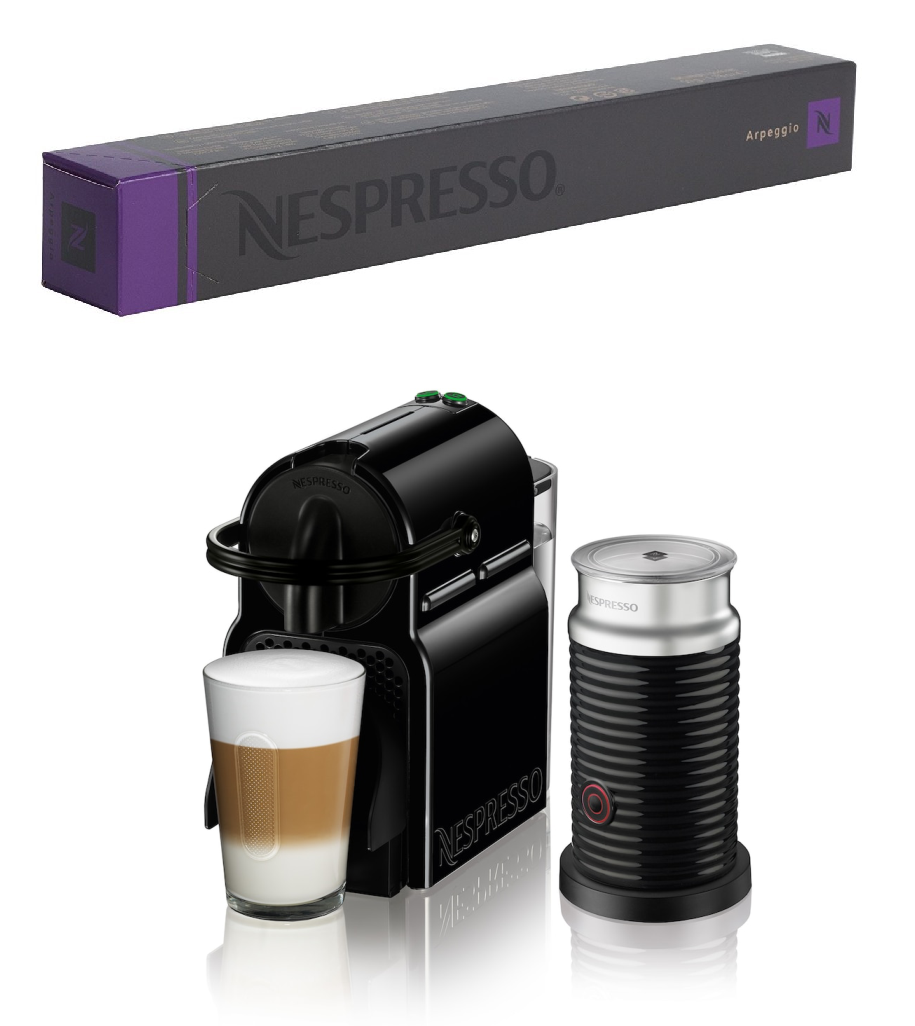
\includegraphics[width=\linewidth]{./figs/02-state-of-the-art/sleeve.pdf}
        \caption{Nespresso coffee sleeve, machine and accessories} 
        \label{fig:sleeve}
    \end{subfigure}
    \begin{subfigure}{.45\textwidth}
        \centering
        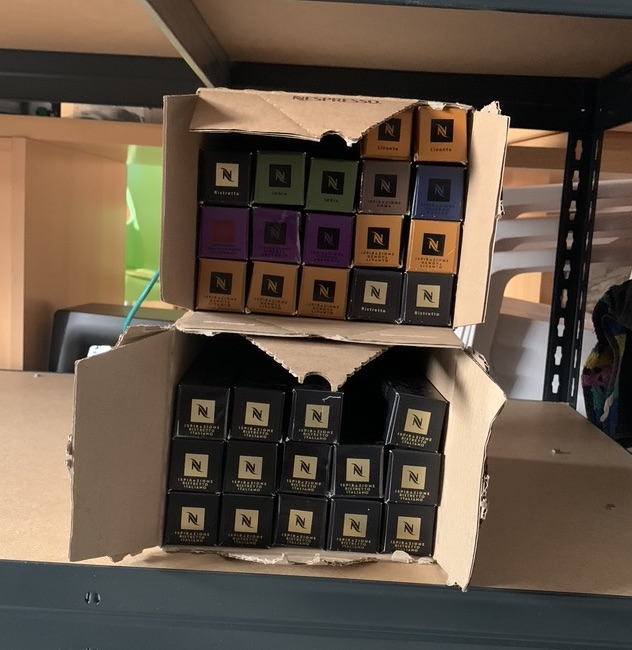
\includegraphics[width=\linewidth]{./figs/02-state-of-the-art/sleeveboxes.jpeg}
        \caption{Nespresso sleeves and outer cardboard packing used in distribution} 
        \label{fig:sleevepacking}
    \end{subfigure}
    \label{fig:sleeves}
\end{figure}

The software platform implementation should be agnostic, in that it runs equally well across multiple platforms. It should be capable of effortlessly integrate with the logistics management software and services used by the company and trading partners.

\section{Solution}

The solution proposed in this dissertation is a system of smart shelving, where the goods like coffee capsules, machines and accessories are stored. These goods are tagged with \ac{rfid} tags and integrated in an \ac{rfid}-enabled supply chain.
The shelve structure contains \ac{rfid} antennas and readers that detect and read the tags attached to the stored products. Readers will send real-time state and changes of inventory to the software platform, which filters and contextualizes the data, stores it, and provides appropriate query interfaces to managing software systems.
This system can solve multiple issues and in the future integrate multiple features like:

\begin{itemize}
    \item Prevent stock-outs and get timely replenishment of products. Logistics companies deliver goods on time and according to delivery requirements generated automatically by a management system;
    \item Reduce time and errors from manual labour: counts, identification, misplacement and lost or stolen items;
    \item Control who removes or checks out valuable products;
    \item Automate information about stock predictions. Manufacturer production lines automatically transmit and receive re-stock interest information.
    \item Handle registration and verification of arriving stock. Automatically identify goods in the warehouse/shelves and match them with distribution invoices;
    \item Verify products trades as goods enter the collection area. The collection equipment automatically identifies items, by collecting \ac{rfid} tags, thereby ensuring the physical and  distribution requirements are consistent;
    \item Monitor in real-time the distribution of all goods, accurately know inventory state and grasp the status and changes of the warehouse environment in real time.
\end{itemize}

In the design and planning of this solution, there are two different contexts considered. The first is how a real product would be designed to be ready for the envisioned environment. Costs, deployment problems and architecture designs should be well thought in order to achieve a stable and commercially appealing product.
The second context is a generic prototype implementation showing a working proof of what the real product would be like.
In a real-world implementation, sleeves would not be tagged, as it would increase significantly operation costs without significant benefits. For academic purposes of studying tag density read performance, each sleeve was tagged.

In the remaining of this chapter I will discuss and show multiple development options: hardware, product design and platform software. In the last section of this chapter, I will present and clarify the options taken to prototype the smart shelve solution accomplished in this dissertation.

\section{\acs{rfid} Technology}

It was clear, early in the researching for this dissertation, that the \ac{rfid} technology which would be used was \ac{uhf}. 
It is the most reasonable option in this context: it has the reading distance requirements necessary for the solution envisioned; it provides the cheapest and best performance tags, with promises of even cheaper, more robust and efficient in the future; and most important, it is the \ac{rf} technology used in \ac{gen2} tags and \ac{scm} systems deployed around the globe. 
Would not make sense to diverge from the well established implementations and difficult the integration in logistics and supply chain systems.
In fact, it would create a technological frontier and incompatibility in respect to tag technology.
With this, there is no further critical incentive to opt for other \ac{rfid} technology other than \ac{uhf} \ac{rfid}.

\section{Readers}

\subsection{Considerations}

To buy commercial readers or make a custom implementation?
The answer is deeply dependent on company long term plans, namely in the balance between \ac{rnd} cost, return on investment, and long term benefits. Compromises in engineering work have to be clearly balanced with the company needs and requirements. If the \ac{rfid} implementation plans extend deeply into the organization - points of sale, distribution centers, warehouses and manufacturing - making a custom reader solution might make sense, when evaluating cost margins and requirements. For companies like Walmart, Decathlon and big retailers, the investment in custom hardware should definitely be considered.

Commercial readers tend to be very expensive. They are usually designed for generic applications, providing incredible reading distances, astonishing number of tag reads per second, and multiple other features to please every client and fit every application.
This makes them rather expensive and excessive for applications like smart shelves.

Smart shelves, in most design approaches, do not require high power transmission nor high tags reads per second. Designs usually take advantage of \ac{rf} splitters and multiplexers to connect multiple antennas. They could also take advantage of WiFi, LTE and PoE capabilities, over the traditional communication interfaces like the serial port.

Returning to the main premise, there are two paths which can be followed: development of a custom reader~\footnote{When I address the development of custom readers, I do not specify who and how, as it can be done by consulting companies or in house. In this dissertation I only discuss development considerations and not how those are translated to engineering work} or adopt a commercial one. 
Custom designs for smart shelves can be much cheaper: less features translate to few hardware requirements; lower power transmission allows cheaper \ac{rf} amplifiers (commercial readers can read up to $10m$, and depending on shelve implementations, we might only require reads up to $1m$); lower requirements in reads speeds allow cheaper \ac{epc} \ac{c1g2} SMD or chip solutions, like \acp{ic} designed for handheld readers, which tend to be less powerful but cheaper.
On top of being cheaper, custom readers allow developers to implement features otherwise nonexistent. Many readers expose interfaces mainly through Java and C\# SDKs. Open standards like \ac{llrp} are usually provided only in few high-end commercial readers. The stagnant condition of commercial readers, also does not keep up with new \ac{iot} and \ac{it} technologies, which have showed to be incredible powerful, mainly in the distributed computing, and dismissed in favor of legacy technologies.
Custom readers can also integrate middleware capabilities (i.g.\ ``smart readers'' conceptualized in the \emph{EPCGlobal Architecture Framework}), and capture application features, encouraging a deprecation of discrete middleware and capture applications in a few contexts.
On the other hand, the development of such readers is \ac{rnd} intensive. For small and medium companies, such option is not remotely reasonable. 
For big companies, this kind of project would certainly be approached by consulting companies, since \ac{rfid} hardware is not within the expertise of most \ac{scm} and retailers. Companies like Nike, Zara and Walmart have built in-house tools and outsourced hardware, strengthening the proposition I am presenting.

\subsection{Market Offer}

The market of RAIN \ac{rfid} \ac{gen2} compatible readers is extensive, but not very divergent in hardware implementations, in that most readers are based on just a few commercial \ac{epc} \ac{c1g2} \ac{ic} chips.

Currently, the \ac{epc} \ac{c1g2} reader chips available on the market are listed on table~\ref{tab:readerchips}.
The considerable market leader is Impinj, which commercializes their own readers and development kits, with their in-house reader chips~\cite{RAINRFIDReader}. Most commercial readers available on the market (e.g.\ CAEN RFID and Jadak ThingMagic modules~\cite{RAINRFIDPartner}) use their chips.
There are other players in the \ac{epc} \ac{c1g2} reader chip market. 
STMicroelectronics acquired Austriamicrosystems' \ac{nfc} and \ac{rfid} reader assets in 2016~\cite{PressRelease}. Austriamicrosystems provided, the now discontinued \texttt{AS3990} (i.g.\ \texttt{ST25RU3991}), \texttt{AS3990} (i.g.\ \texttt{ST25RU3992}) and \texttt{AS3980} (i.g.\ \texttt{ST25RU9080}) used by academics to create cheap \ac{c1g2} readers~\cite{tangDesignUHFRFID2010a, leiDesignHandheldUHF2011, liDesignRadioFrequency2011}. Currently STMicroelectronics
commercializes their \texttt{ST25RU3993} chip~\cite{ST25RU3993}, used in their evaluation boards and in few commercial readers, like Feig's~\cite{UHFMidRange}.
There are also companies selling \ac{epc} \ac{c1g2} SMD reader/writer modules, namely Nordic, with the ID NUR~\cite{NURModulesNordic}, and ThingMagic with the M6e, Micro and Nano~\cite{ThingMagicRFID}.

\begin{table}
    \centering
    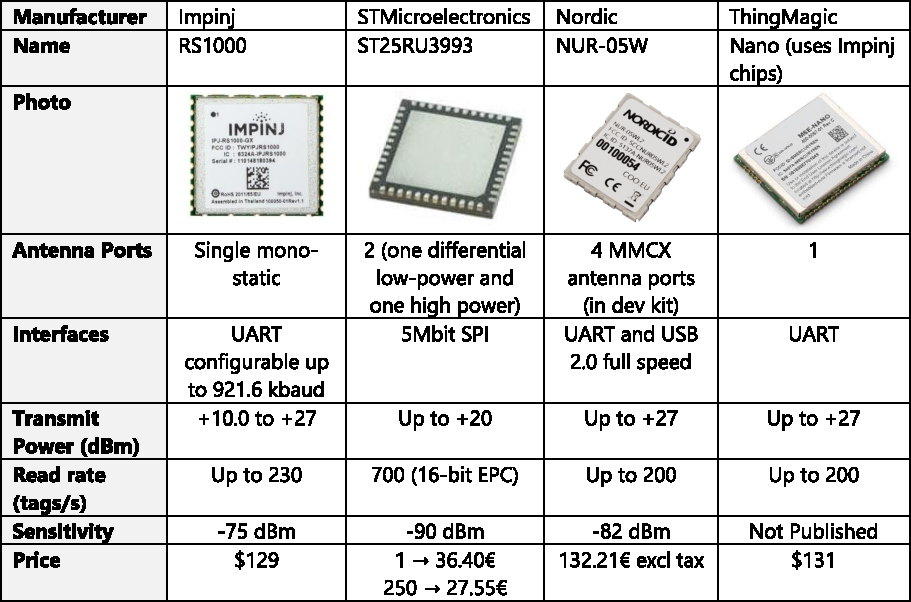
\includegraphics[width=\linewidth]{./figs/02-state-of-the-art/table_chipreaders.pdf}
    \caption[Available \ac{epc} \acs{c1g2} reader chips and SMD modules on the market]{Available \ac{epc} \acs{c1g2} reader chips and SMD modules on the market. Information and prices gathered from respective datasheets, AtlasRFIDstore~\cite{AtlasRFIDstoreBuyRFID} and Mouser~\cite{DistribuidorComponentesEletronicos}.}
    \label{tab:readerchips}
\end{table}

\begin{figure}[H]
    \centering
    \begin{subfigure}{.35\textwidth}
        \centering
        \includegraphics[width=\linewidth]{./figs/02-state-of-the-art/impinjrs1000.pdf}
        \caption{Impinj RS1000 development kit (End-of-Life announced on September 4, 2020)} 
        \label{fig:impinjrs1000}
    \end{subfigure}
    \begin{subfigure}{.55\textwidth}
        \centering
        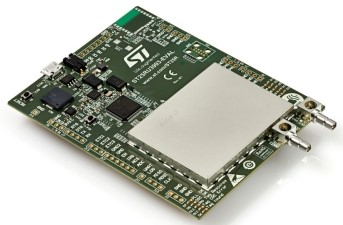
\includegraphics[width=\linewidth]{./figs/02-state-of-the-art/st25ru3993-eval.jpg}
        \caption{STMicroelectronics ST25RU3993 evaluation board (\$306.25 at Digikey)} 
        \label{fig:st25ru3993}
    \end{subfigure}
    \label{fig:devboards}
\end{figure}

Regarding commercially available readers, there is an extensive variety of solutions, too many to discuss in this dissertation. An overview of established, widely deployed readers can be seen in table~\ref{tab:readercommercialsolutions}.
Alien Technology, has been commercializing their own \ac{rfid} readers~\cite{AlienTechnologyReaders} for years, having a well established client base. Impinj, Fujitsu, Honeywell, ZIH Corp, Mitsubishi, Omron, Takaya, Toshiba, Tyco Sensormatic and Zebra also have \ac{epc} \ac{c1g2} reader solutions, most of them with \ac{llrp} interfaces.

\begin{table}
    \centering
    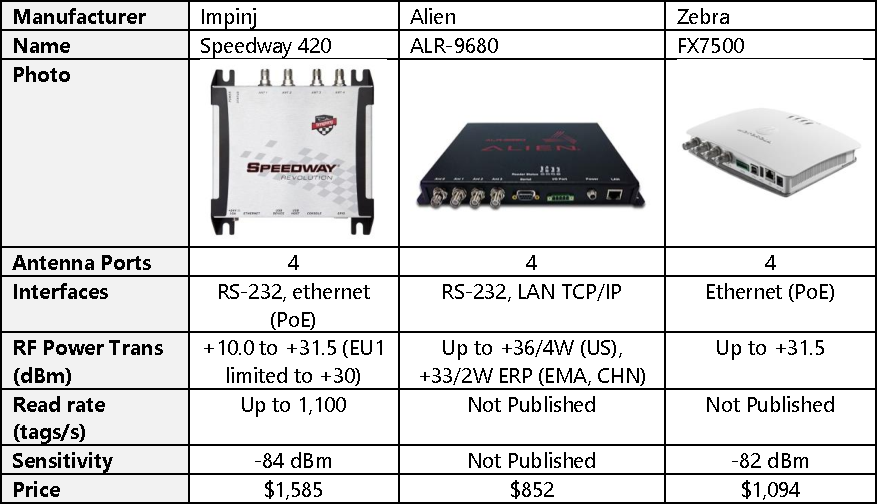
\includegraphics[width=\linewidth]{./figs/02-state-of-the-art/table_commercialreaders.pdf}
    \caption[\ac{epc} Class 1 \ac{gen2} compatible readers well established on the market]{\ac{epc} Class 1 \ac{gen2} compatible readers well established on the market. Information and prices gathered from respective datasheets and AtlasRFIDstore~\cite{AtlasRFIDstoreBuyRFID}.}
    \label{tab:readercommercialsolutions}
\end{table}


\section{Antennas}

The discussion between custom and commercial readers made previously, can also be transposed to the selection of antennas. In certain conditions, the development of custom solutions can present good incentives.

Most smart shelves implementations, require mainly antenna designs tunned for the \ac{em} \emph{near-field} region.
In section~\ref{sec:academicsolutions}, I cited numerous implementations of \emph{near-field} \ac{uhf} \ac{rfid} antennas, intended to be used in smart shelves and similar purposes, by the academic personnel. Many of these present suitable performance to be integrated in smart shelve systems, are simple, easy to manufacture and are much cheaper than commercial alternatives. 

Regarding commercial availability solutions, the market offers generic high performance antennas and designs for most applications, having a wider range of specific, single-purpose products, compared to the \ac{uhf} reader market. 
High performance antennas tend to be expensive due to the strong requirements in reading distances. Single-purpose antennas are also expensive, intrinsic to their narrower market share. 
In table~\ref{tab:antennasolutions} it is shown a few compact commercial antennas considered for the implementation of this dissertation.

\begin{table}
    \centering
    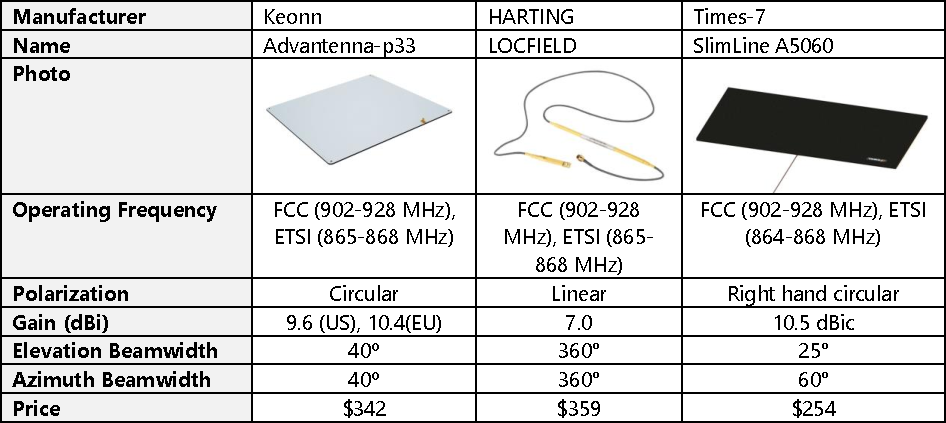
\includegraphics[width=\linewidth]{./figs/02-state-of-the-art/table_antennas.pdf}
    \caption[A few \ac{uhf} \ac{rfid} compact antennas available on the market]{A few \ac{uhf} \ac{rfid} compact antennas available on the market. Information and prices gathered from respective datasheets and AtlasRFIDstore~\cite{AtlasRFIDstoreBuyRFID}.}
    \label{tab:antennasolutions}
\end{table}

When selecting antennas, it is important to take in consideration their polarization. Systems where the tag orientation is unpredictable, which is the case of most smart shelves, the selection of circular antennas is desireable. Alternatively, two or more linear antennas can be used to mitigate the orientation problem.
Even with circular antennas, tag orientation can affect readings in certain conditions, being advisable to prototype and test with different antenna models and placement, in extreme operational conditions.

The approach taken in antenna selection is similarly to reader selection, in that it depends on company approach to such endeavor and product design, which I will be discussing next.

\section{Architectural Design}

Smart shelves can be implemented and designed in different manners, varying in number of antennas, their position, size and power transmitted.
D’Alessandro, in his PhD thesis~\cite{dalessandroRFIDBasedSmartShelving2012}, prototyped and evaluated a few possible implementations, which were taken in consideration in planning and designing the shelf developed in this dissertation.
In this section I will present a few architectural designs for \ac{uhf} \ac{rfid}-enabled smart shelves, how they differ, and discuss a few implementation considerations.

The first design, shown in figure~\ref{fig:position1}, is the simplest of all. It can be implemented with a single reader and two antennas. The figure shows a top view of a shelve with an external antenna, radiating at an angle. Variations of this design can be found in retail stores, with ceiling antennas pointing to shelves.
The simplicity and functionality of this design is what makes it appealing and fairly adopted.
Problems in this arrangement emerge mainly due to tag-to-tag interference and \ac{rf} obstruction zones, which can appear due to interference from certain materials (see table~\ref{tab:rfproperties}).

With two antennas at different angles, it is possible to locate objects with decent accuracy, using metrics~\footnote{Most commercial readers provide \ac{rf} metrics like \ac{rssi}, \ac{toa}, \ac{aoa}, \ac{pdoa}} provided by readers, and classification algorithms, using reference tags attached to strategic places of the shelves~\cite{dalessandroRFIDBasedSmartShelving2012}.

\begin{figure}[H]
    \centering
    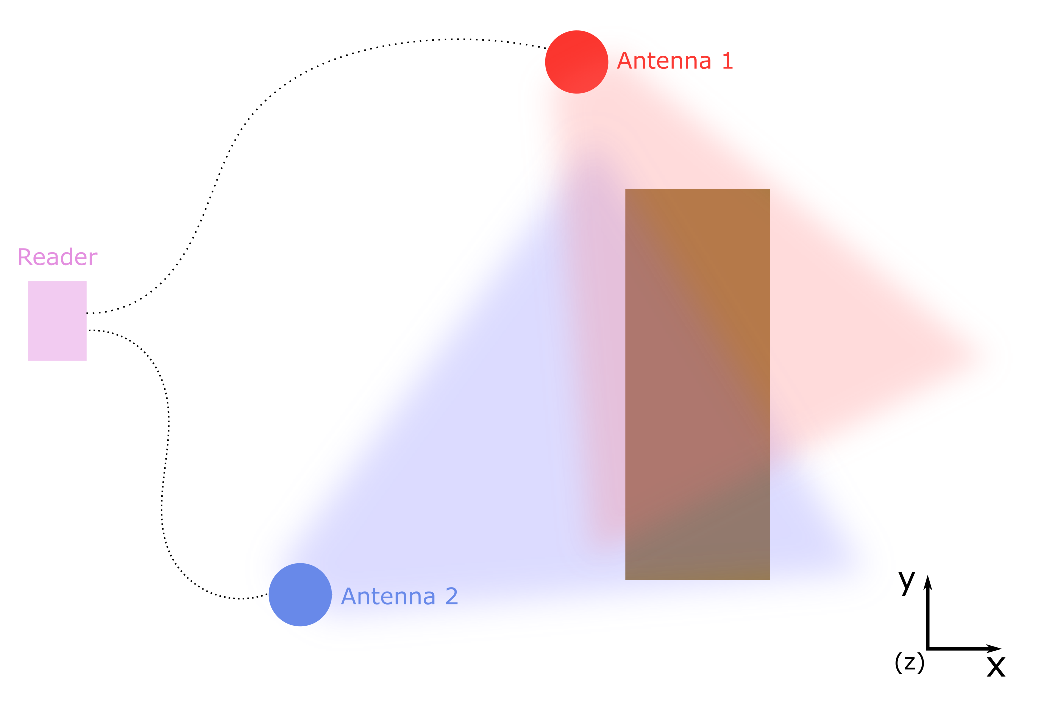
\includegraphics[width=0.6\linewidth]{./figs/02-state-of-the-art/position1.eps}
    \caption{Top view of two external antennas radiating a shelve at different angles}
    \label{fig:position1}
\end{figure}

Figure~\ref{fig:position2} shows the most frequent approach when designing smart shelves, by placing one or multiple compact antennas in each shelf.
These antennas can be incorporated into a shelf, making it invisible and ideal for point of sale in retail stores.
Reading zones can be very precisely distributed, creating less \ac{rf} ``polution'', desirable in contexts like shared warehouses in malls, where other \ac{rfid} system might be deployed.
The location techniques described in the first arrangement can be adapted and implemented in similar manner in this design.

This implementation has the downside of requiring multiple antennas, usually connected to a reader by \ac{rf} splitters and multiplexers.
These hardware requirements make this design fairly expensive, being a good example of where custom hardware design is encouraged.

This design has been used in products like the ones in chapter~\ref{sec:smartshelves}, library management shelf systems~\cite{markakisSafeEfficientDesign2014} and in smart lockers.

\begin{figure}[H]
    \centering
    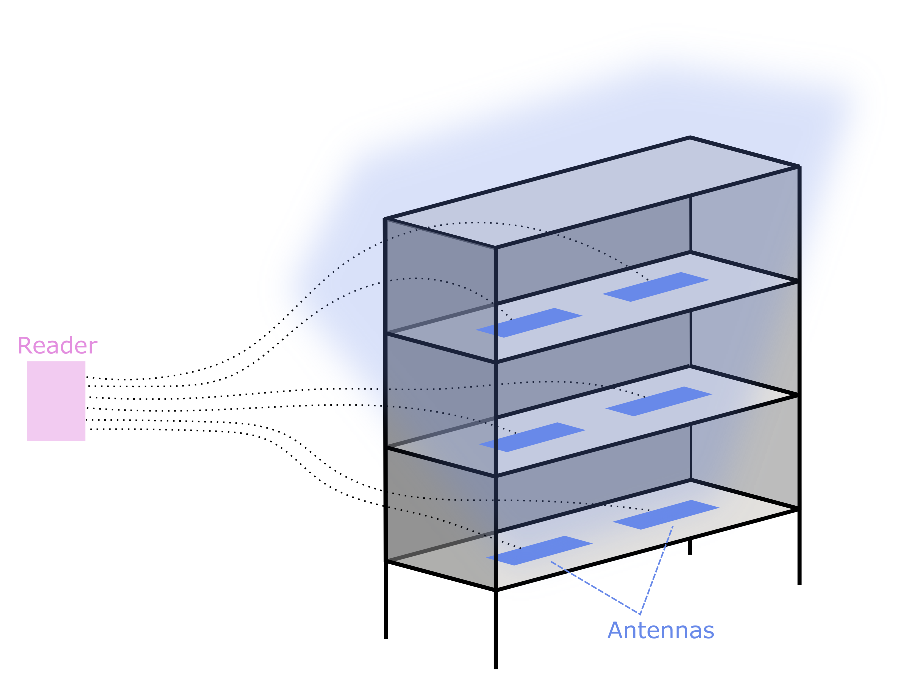
\includegraphics[width=0.6\linewidth]{./figs/02-state-of-the-art/position2_1.eps}
    \caption{Arrangement with multiple compact antennas distributed in each shelf radiating upwards} 
    \label{fig:position2}
\end{figure}

In conclusion, the last arrangement we will discuss is shown in figure~\ref{fig:position3}. It places two antennas per shelf, one in each side of opposing laterals. This approach can be implemented without the use of necessarily compact antennas and favors long shelf designs.
This design has been used primarily in library shelf implementations~\cite{markakisRFIDenabledLibraryManagement2013}.

Similarly to the last design, it presents the downside of requiring multiple reader ports or \ac{rf} multiplexers. Uniquely to this design, it requires to have antenna designs tuned for both \emph{far} and \emph{near-fields}.

\begin{figure}[H]
    \centering
    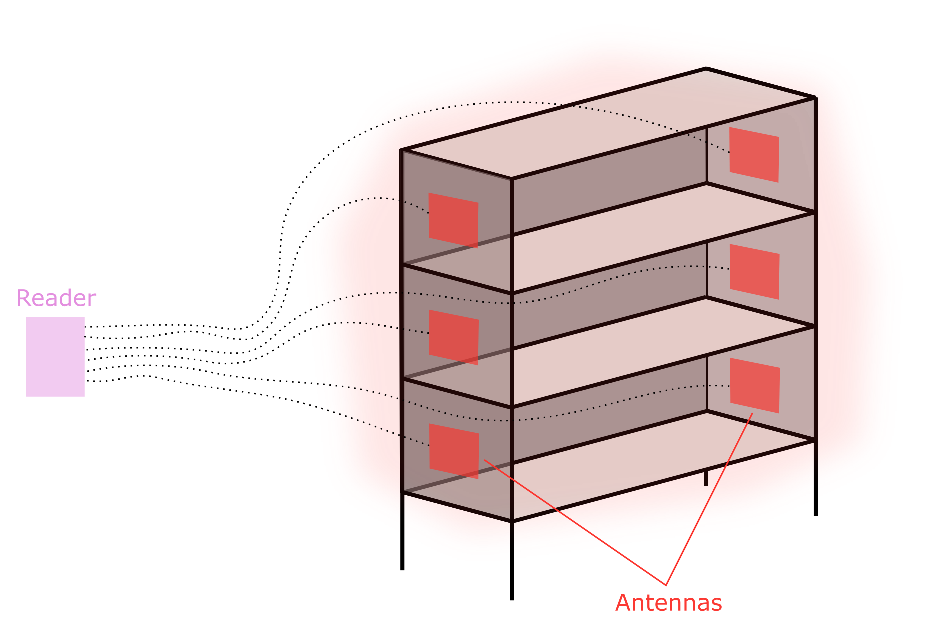
\includegraphics[width=0.6\linewidth]{./figs/02-state-of-the-art/position3.eps}
    \caption{Arrangement with two antennas per shelf, one in each side of opposing laterals radiating inwards} 
    \label{fig:position3}
\end{figure}

\section{Software}

\subsection{Reader Interface Software}

Interaction with \ac{uhf} readers is uniform across the industry.
Reader manufacturers generally make Java, C$++$ and C\# SDKs available for commercial and chips reader solutions. These SDKs allow integrators to configure and interact with these through high level APIs, which usually abstract the \ac{gen2} air protocol. SDKs can also expose low level APIs to precisely control the reader and tune the air protocol.

\ac{llrp}-compliant readers can use \ac{llrp} client programs, like the Fosstrak LLRPCommander~\cite{FosstrakLLRPCommander}, based on Eclipse 3.3, to manage and receive tag information. 
There are also libraries available to decode and encode \ac{llrp} messages, which can be used to make \ac{llrp} clients. A few of those worth mention: \texttt{sllurp} and \texttt{pyllrp} implemented in Python, \ac{llrp} Toolkits (LTKs) in Java, Perl and C\+\+~\cite{LlrpOrga} and \texttt{go-llrp} implemented in Golang.

To encode, decode and translate \acp{epc} data, there are many available libraries, namely, used in this dissertation, the \texttt{epc-standards} \ac{epc} decoding Java library from Nike~\cite{NikeIncEpcstandards2019}, and Fosstrak Java \ac{tdt} Engine~\cite{FosstrakTagData}.

\subsection{Software Platform} \label{sec:softwareplatformoptions}

The availability of software resources for the \emph{EPCGlobal Architecture} is very limited.
For years, the only software came from Fosstrak Open Source \ac{rfid} Software Platform, which provided an \ac{ale} \ac{fc} Middleware, Capturing Application and \ac{epcis} Repository implementations. Fosstrack last commits to most of the projects dates back 5 years. The technology is outdated, with bugs, documentation errors and the project forum is ``dead''.

Oliot is a fork of the Fosstrak components, which extends GS1 standard architecture to support various \ac{iot} connectivity and protocols such as bar code, ZigBee and 6LoWPAN~\cite{OpenLanguageInternet}. Inherent to being based on Fosstrak code, it suffers, to certain degree, of the same problems and bugs as Fosstrak services.

Iori Mizutani, in this dissertation~\cite{mizutaniRobustHighPerformance} and research~\cite{mizutaniMulticodePortableRFID2016b}, has contributed with a modern implementation of a \ac{fc} middleware (\href{https://github.com/iomz/gosstrak}{\texttt{gosstrak}}) and reader emulator (\href{https://github.com/iomz/golemu}{\texttt{golemu}}) in Golang~\cite{mizutaniIomzGolemu2020, mizutaniIomzGosstrak2020}. 
His work seems promising in the nonexistent contribution to the EPCGlobal standards in the last years. Although, his \ac{fc} implementation is not production ready. The project is not actively maintained anymore, only implements a simplified version of the \ac{ecspec} and the \ac{ale} interface provided is incomplete.

IoTA supplies EPCGlobal tools in their ecosystem of distributed technology~\cite{GlobalTradeSupply}. It uses Fosstrak components and adds a prototype of the Discovery Service and secured \ac{epcis} components~\cite{FosstrakSimilarProjects}. Their platform integrates distributed networks, block-chain, micropayments, immutable data and many other technologies which reach far out the scope of this dissertation.

Commercial EPCGlobal solutions are usually not provided as a single product or service. Consulting companies generally provide their services in a solution bundle.

Ricoh commercializes a software middleware \ac{fc} solution called RECO-Bridge IDR-1 V2. It sells for $850000$ yen ($\approx 6736$€) and is operated in Microsoft® Windows Server™. Offers filter capabilities, monitoring functions for \ac{rfid} systems, provides \ac{ale}-complied interfaces, can connect and control up to $32$ \ac{uhf} and/or \ac{hf} reader/writers~\footnote{up to $64$ if purely using \ac{hf} reader/writers} and $128$ antenna units using \ac{llrp} v$1.1$ protocol interface~\cite{RECOBridgeIDR1V2}.

Quake Global Inc. commercializes the EasyTap™ \ac{rfid} middleware~\cite{EasyTAPRealTime}. Their web page advertises multiple data services and application integration standards, traffic visualization in real-time and performance optimization capabilities. External sources specify a little further the capabilities of their EasyTAP751 hardware solution seen in figure~\ref{fig:easytap751}. It supports \ac{llrp}, provides \ac{ale} and \ac{epcis} data capture interfaces~\cite{RFIDEasyTAPTag}.

\begin{figure}[H]
    \centering
    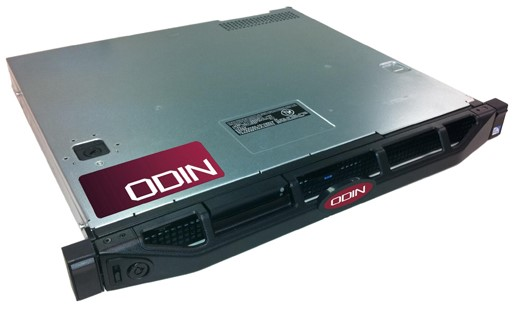
\includegraphics[width=0.6\linewidth]{./figs/02-state-of-the-art/easytap751.jpg}
    \caption[Quake Global Inc. EasyTAP751 middlware hardware solution]{Quake Global Inc. EasyTAP751 middlware hardware solution~\cite{RFIDEasyTAPTag}} 
    \label{fig:easytap751}
\end{figure}

Transcends commercializes the RIFIDI® Edge Server middleware software solution~\cite{RIFIDIEdgeServer2015}. It supports \ac{llrp} and integrates with most \ac{iot} protocols and cloud vendors (e.g.\ REST, MQTT, JMS, ALE, AWS, Cloud). Does not specify EPCGlobal integration or interfaces. It costs \$$3000$ in 1st year, \$$2000$ each consecutive year, per JVM instance up to 10 readers, with 5\% price increase for each additional JVM.

\section{Our choice} \label{sec:ourchoice}

\subsection{Context}

Before proceeding with the discussion on the opted choice of hardware and software, a brief contextualization is needed.
The introductory proposal for this dissertation was not clearly defined in terms of objectives and work. The downright agreement was to develop a generic smart shelf solution based on \ac{rfid} technologies. The application could vary, and was to be used and adapted in a multitude of contexts like lockers and cabinets.

The initial investigation of the literature focused in a set of topics, which would not be directly used in this dissertation.
First, it was conducted an exploration of \ac{rfid} technologies, in order to determine a suitable \ac{rf} system. It was clear, from early in the study, that \ac{uhf} \ac{rfid} would be the most suitable option. The market of \ac{uhf} had evolved significantly over the years, tags were cheap, performance was better than alternatives and every \ac{scm} deployed was using it. This established confidence in choosing \ac{uhf} \ac{rfid} has the technology to integrate in solution.

With the \ac{rfid} technology determined, I proceeded to study implementation approaches. This prompt research in in \ac{uhf} antenna design, with attention to manufacturing cost. The fact of smart shelves requiring antennas with specifications fairly distinct from available \ac{scm} solutions, fulled this research endeavor.

In parallel, an analysis of available readers and requirements was conducted.
Readers did not provide sufficient antenna ports to handle the multiple antennas required in most smart shelf designs.
For a few application contexts, namely lockers constructed of metal, the poor \ac{rf} conditions caused by the material, imposed a high number of small antennas. The four antenna ports, provided by most commercial readers, were insufficient. 
Alternatively, it could be used \ac{rf} splitters and multiplexers to connect large number of antennas. This alternative was highly expensive.

Later, the exploration of \ac{scm} operations and standards, revealed the \emph{EPCGlobal Architecture Framework}. The architecture was extensive, with many details and technicalities, which took a long time to understand and filter for the use case of this dissertation.
The inexistent research in developing EPCGlobal compliant products motivated the final proposal of this dissertation.

\subsection{Implementation Design and Hardware}

In the final agreement of this dissertation, it was decided to develop a simple generic smart shelf based on \ac{uhf} \ac{rfid} technologies, implementing the necessary EPCGlobal services, standards and interfaces, to achieve a solution where added and removed items could be monitored through a management application.
The implementation of the smart shelf had to be simple and cost limited. 
Due to time constrains, the development of custom hardware had to be avoided in favor of the \emph{EPCGlobal Architecture Framework} implementation.

The shelf used was a $176\times160\times60cm$cm MDF and metal construction, shown in figure~\ref{fig:commercialshelve}. It was chosen for the similarity with most warehouse storage shelves. Was also interest of this dissertation to evaluate real world performance in shelves with metal structures, to study how it interferes with the \ac{emw} generated by the reader antenna.

\begin{figure}
    \centering
    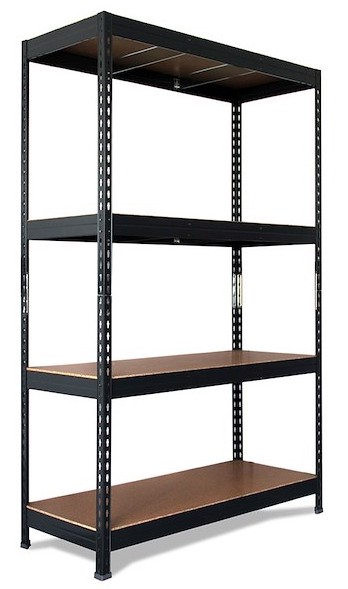
\includegraphics[width=0.4\linewidth]{./figs/estantedemetal.jpg}
    \caption[Leroy Merlin $176\times160\times60cm$cm MDF and metal construction shelve]{Leroy Merlin $176\times160\times60cm$cm MDF and metal construction shelve~\cite{EstanteMetalStabil}} 
    \label{fig:commercialshelve}
\end{figure}

The \ac{rfid} design solution, chosen for the smart shelf, consists of a single compact antenna and reader attached to the bottom shelf, radiating upwards.

The chosen antenna was a Keonn Advantenna-p14, shown in figure~\ref{fig:advantennap14}. This antenna integrates the same technology group and design as Keonn solution of compact antennas for smart shelves presented in section~\ref{sec:keonnsolutions}.
The antenna can radiate the entire shelf, with a $30^{\circ}$ beam width in the direction of the antenna long edge and $90^{\circ}$ in the direction of the antenna short edge, as shown in figure~\ref{fig:advantennap14-radiation}.

\begin{figure}
    \centering
    \begin{subfigure}{.45\textwidth}
        \centering
        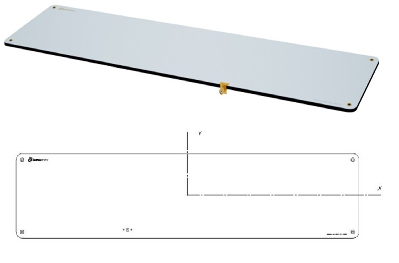
\includegraphics[width=\linewidth]{./figs/advantennap14.pdf}
        \caption{Photography of the Keonn Advantenna-p14. The direction of the antenna long edge is the $x$ axis, the antenna short edge is the $y$ axis} 
        \label{fig:advantennap14}
    \end{subfigure}
    \begin{subfigure}{.45\textwidth}
        \centering
        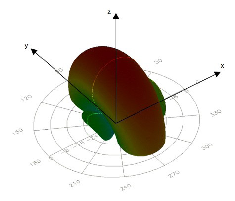
\includegraphics[width=\linewidth]{./figs/advantennap14-radiation.pdf}
        \caption{Radiation diagram of the antenna} 
        \label{fig:advantennap14-radiation}
    \end{subfigure}
    \caption[Keonn Advantenna-p14]{Keonn Advantenna-p14~\cite{Advantennap14RFIDCompact}} 
    \label{fig:antennachoice}
\end{figure}

The reader chosen was the Impinj Speedway R120, shown in figure~\ref{fig:impinjr120}. It is a less powerful, 1 antenna port version of the R420 shown in table~\ref{tab:readercommercialsolutions}. It was chosen for being widely used, has good documentation, tools, state of the art technology, PoE, and most important, provides an \ac{llrp} interface~\footnote{Impinj is one of the big supporter of the \ac{llrp} protocol as an open source interface for \ac{rfid} readers~\cite{SevenRFIDOrganizations}}.

\begin{figure}
    \centering
    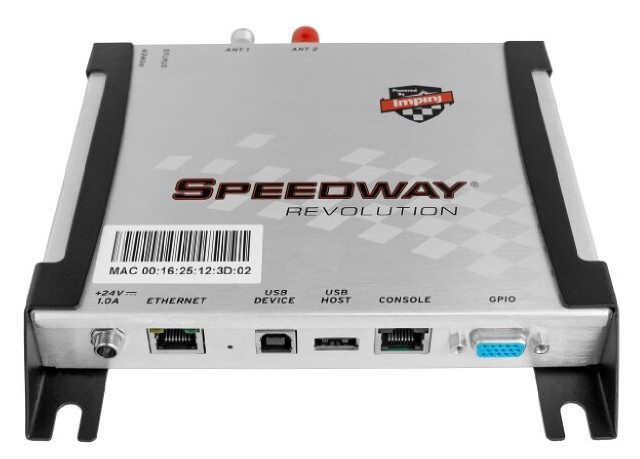
\includegraphics[width=0.6\linewidth]{./figs/Speedway_Revolution_R120.jpg}
    \caption[Impinj Speedway R120 reader]{Impinj Speedway R120 reader~\cite{ImpinjSolucoesRAIN}} 
    \label{fig:impinjr120}
\end{figure}

This combination provides very decent performance, without great investment in commercial and custom hardware. Some problems arise from this implementation, mainly with \ac{rf} obstructions. Performance will be examined in chapter~\ref{sec:tests}.  

Regarding tag choices, it is out of the scope of this dissertation. It was used generic HID 6H2E43 tags~\cite{HidetiquetasrfidPdf}, shown on figure~\ref{fig:6H2E43}.
These tags use Impinj Monza R6-P chips with 96 bit \ac{epc} and 32 bit \ac{umi}. They are made of PET material, with a size of $92\times28$mm and reading distance up to $14$m.

\begin{figure}
    \centering
    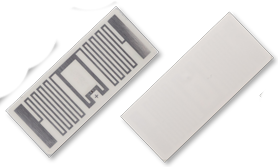
\includegraphics[width=0.6\linewidth]{./figs/6H2E43.png}
    \caption[HID 6H2E43 $92\times28$mm PET tag with $96$ bit \acs{epc}]{HID 6H2E43 $92\times28$mm PET tag with $96$ bit \acs{epc}~\cite{EtusivuIDcontrol}} 
    \label{fig:6H2E43}
\end{figure}

To program the reader and evaluate its operation, it was used the Octane Java SDK provided by Impinj. 
The SDK uses the Octane \ac{llrp} LTK, as the base library. The Octane \ac{llrp} LTK is an extension of the open source LTK implementation, with added Impinj commands, extensions and features.
The Octane SDK high level API design captures fairly well the \ac{llrp} essence, making it intuitive, with knowledge of the protocol, to understand which \ac{llrp} messages are traded and what they contain.

Regarding the development of the platform, great effort was given to make the EPCGlobal services fairly modular and modern, despite the very old software it runs.
Fosstrak Open Source \ac{rfid} software services were chosen. Alternatives only seemed to complicate and widen the platform with unnecessary features. The problems shown in Fosstrak are also present in the alternatives, which use Fosstrak code.
Docker was used to containerize services. 
Docker packages up code and all its dependencies in what is called a container, which allows applications to run quickly and reliably from one computing environment to another. Docker containers can be easily deployed and managed in all major cloud computing platforms, and are widely used in the current paradigm of cloud computing.
Docker compose was used to orchestrate the containers and networks locally for testing.

In the next chapter we will get in to the details of the configuration of the reader and platform services.
